\chapter{Implementation}

This section provides a comprehensive account of the design and functional integration of the proposed system, which leverages Retrieval-Augmented Generation (RAG) and Agentic Artificial Intelligence (AI) to replace conventional regular expressions in pattern extraction tasks. The discussion encompasses the system's architectural framework, dynamic operational workflow, and the autonomous behavior of its constituent agents.

\section{Architecture of the System}
The architecture of the proposed system, which integrates Retrieval-Augmented Generation (RAG) and Agentic Artificial Intelligence (AI), is designed in a modular and layered manner to ensure flexibility, scalability, and adaptability. The system comprises five primary components, each dedicated to a specific function within the overall process and execution pipeline: (see Figure~\ref{fig:agentic_rag})


\subsection{Input Interface}
This module serves as the entry point of the system, responsible for receiving natural language prompts from the user and transforming them into structured requests. It performs language type validation, extracts task intent through a preliminary parsing mechanism, and subsequently forwards the refined input to the RAG subsystem for further processing.

\subsection{RAG Module (Retriever + Generator)}
This component constitutes the core of the Retrieval-Augmented Generation (RAG) mechanism. It utilizes FAISS for dense vector retrieval, enabling efficient access to relevant documents, examples, or knowledge snippets based on the user's query. The retrieved content is then supplied to a generative language model (e.g., GPT-4 Turbo or Gemini-Pro), which synthesizes the contextual information into high-level intent representations or pseudo-code approximating a pattern extraction strategy.


\begin{figure}[h!]
    \centering
    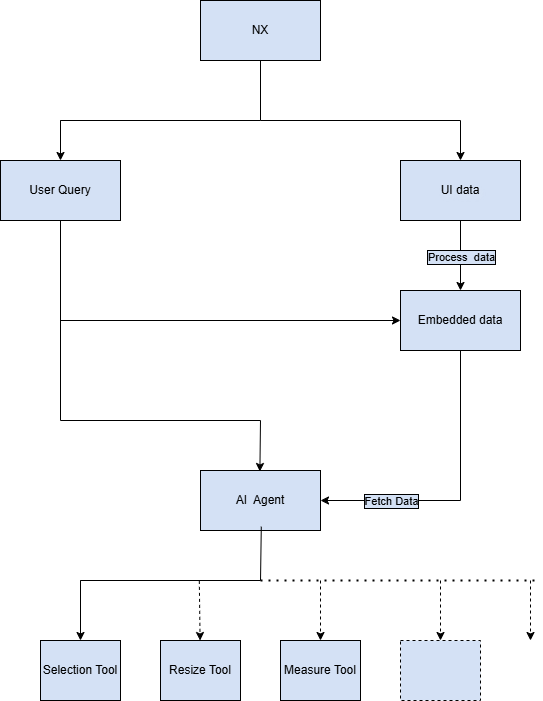
\includegraphics[width=0.95\textwidth]{images/NX_Diagram.drawio.png}  % Use relative path for portability
    \caption{System Architecture: Agentic RAG Framework and Component Stack. The diagram illustrates the modular flow from user input through RAG retrieval and generation, agentic planning, tool execution, and output integration.}
    ~\label{fig:agentic_rag}
\end{figure}



\subsection{Agent Planner}
The agent planning module, implemented using LangGraph~\cite{langgraph2024agentai}, is tasked with formulating a step-by-step execution strategy. It decomposes high-level intent into discrete subtasks, maintains an internal planning state, and dynamically selects appropriate tools for execution. The planner is memory-aware and incorporates reflection-based adaptation mechanisms to revise plans in response to task failures or unexpected outcomes.


\subsection{Tool Executor Layer}
This layer encompasses a suite of APIs and logic modules responsible for executing the subtasks generated by the agent planner. It includes tools such as regular expression compilers, pattern validators, JSON/XML parsers, HTML tag extractors, and text normalization utilities. Each tool is encapsulated with a response handler that provides execution feedback, including success or failure status, confidence scores, and detailed execution logs.


\subsection{Feedback Engine}
In the current implementation, the feedback and recovery process is conducted through manual testing rather than an automated feedback loop. Human evaluators monitor the system's outputs to assess the success or failure of pattern extraction tasks. Upon detecting errors—such as failed matches or incorrect formatting—the evaluator manually traces the tool outputs to identify bottlenecks or missteps and adjusts input configurations or tool selections as needed. This manual evaluation approach ensures rigorous validation and facilitates iterative refinement of the system's orchestration logic and tool effectiveness.

% \vspace{2.0cm}

\section{Workflow: Perception, Planning, Retrieval, Action}
The proposed system employs a cognitively inspired, step-wise workflow that emulates human reasoning and decision-making processes. This workflow consists of five tightly integrated stages—Perception, Planning, Retrieval, Action, and Reflection—which collectively enable the system to dynamically and adaptively interpret user instructions and execute complex pattern extraction tasks with contextual awareness and operational flexibility.


\subsection{Perception}
Perception constitutes the initial stage of the system and forms the foundation for task comprehension. This stage involves capturing the user's natural language instruction and analyzing it to extract semantic content and actionable intent. The process encompasses the following steps:
\begin{itemize}
    \item Text normalization and tokenization, which decompose the instruction into machine-readable units.
    \item Semantic parsing to discern whether the user’s request involves data matching, transformation, validation, or a combination thereof.
    \item Intent classification to identify whether the extraction target is structural (e.g., extracting fields from JSON), pattern-based (e.g., emails, timestamps), or semantic (e.g., dates mentioned within a sentence).
\end{itemize}
The output of this stage is a structured task representation that guides subsequent planning and tool selection.


\subsection{Planning}
Following task comprehension, the agent initiates the planning phase, wherein high-level goals are decomposed into actionable and executable steps. The planning process includes:

\begin{itemize}
    \item \textbf{Task decomposition}: Dividing the overall problem into smaller, manageable subtasks, such as identifying a pattern, applying regular expressions, and validating the extraction results.
    \item \textbf{Sequencing}: Determining the optimal order for executing these subtasks to maximize efficiency and accuracy.
    \item \textbf{Tool mapping}: Assigning each subtask to the most appropriate tool(s) available within the system, such as selection tool, measure tool, highlight tool etc.
\end{itemize}

The planning mechanism is dynamic and iterative; in the event of tool failure during execution, the planner can reconfigure the strategy based on feedback derived either from human evaluators or internal agentic memory.



\subsection{Retrieval}
This stage leverages the Retrieval-Augmented Generation (RAG) framework and plays a critical role in grounding the agent’s reasoning process. Instead of relying exclusively on the inherent knowledge of a pre-trained large language model (LLM), the system queries an indexed document corpus using FAISS to retrieve relevant information, including:

\begin{itemize}
    \item Examples of analogous pattern extraction tasks,
    \item Documentation or schema references pertinent to the expected data format,
    \item Sample regular expressions or validation logic derived from prior interactions.
\end{itemize}

The retrieved materials are subsequently input to the LLM, which integrates this contextual information to generate intermediate instructions or enhancements. For example, in cases of task ambiguity, the retrieval process aids disambiguation by providing contextual data aligned with previous tasks or documented standards.


\subsection{Action}
The action phase represents the execution stage, during which the agent operationalizes the plan by invoking the selected tools. This process involves:

\begin{itemize}
    \item Calling the appropriate modules, such as selection tool or measure tool,
    \item Providing these tools with the necessary input and detailed instructions derived from the plan,
    \item Logging and capturing tool outputs, execution durations, and success or failure indicators.
\end{itemize}

Each tool functions as an independent microservice, returning results accompanied by a confidence score. For instance, when extracting dates from a noisy email dataset, the system may employ multiple regular expression tools and subsequently select the output with the highest match accuracy and contextual relevance.


\subsection{Reflection}
When the system's output deviates from the expected format or fails to meet validation criteria, the agent transitions into the reflection phase. During this stage, the agent:

\begin{itemize}
    \item Consults its short-term memory to reassess preceding steps,
    \item Analyzes which tool underperformed or failed and identifies the underlying causes,
    \item Determines whether to retry with adjusted tool parameters or to revise the planning sequence.
\end{itemize}

In the current implementation, this reflective process is supplemented by manual testing, wherein human evaluators review the outcomes, document the types of failures encountered, and modify system configurations or agent behaviors accordingly. Such human-in-the-loop interventions function both as validation mechanisms and as drivers for the iterative refinement of the agent’s decision-making pathways.










